% 01-introduction.tex — Introduction générale (≈ 4 pages).

\chapter{Introduction}
\label{chap:introduction}

\section{Contexte}

\begin{arediger}{1 page}
Le cours de Physique~1 en première année d'ingénieur civil : public nombreux,
hétérogène, transition secondaire–université. La mécanique newtonienne
(cinématique, dynamique, énergie, mouvement circulaire) est la première
rencontre avec une physique formalisée. Constat de terrain du professeur :
les étudiants manipulent les formules sans se représenter les forces
(exemple du looping : \enquote{la force centrifuge pousse la bille vers
l'extérieur}). Citer \textcite{hestenes1992fci} et \textcite{hake1998}.
\end{arediger}

\section{Problématique et questions de recherche}

\begin{arediger}{1 page}
Question principale : des simulations interactives conçues pour le cours, qui
montrent en même temps le phénomène, les forces et les formules avec leurs
valeurs numériques, améliorent-elles la compréhension des étudiants de BAC1 ?
Sous-questions : (1) quelles caractéristiques de conception comptent
(représentations liées, contrôle du temps, ludification) ; (2) un enseignant
peut-il produire de telles simulations avec un assistant de programmation
fondé sur l'IA, à un niveau de qualité vérifiable ; (3) quel est l'effet
mesuré sur l'apprentissage et la motivation. Formuler les hypothèses
testées au chapitre~\ref{chap:protocole}.
\end{arediger}

\section{Démarche et contributions}

\begin{arediger}{1 page}
Présenter le site (figure~\ref{fig:intro-accueil}) : quatre à cinq exercices
de mécanique, tous construits sur le même gabarit ; un mode jeu expérimental ;
une méthode de développement assistée par IA reproductible ; un protocole
d'évaluation. Énoncer clairement ce qui est original : la combinaison
formules substituées pas à pas + diagramme des forces + jeu dont la condition
de réussite est la relation du cours (chapitre~\ref{chap:jeu}).
\end{arediger}

\begin{figure}[ht]
  \centering
  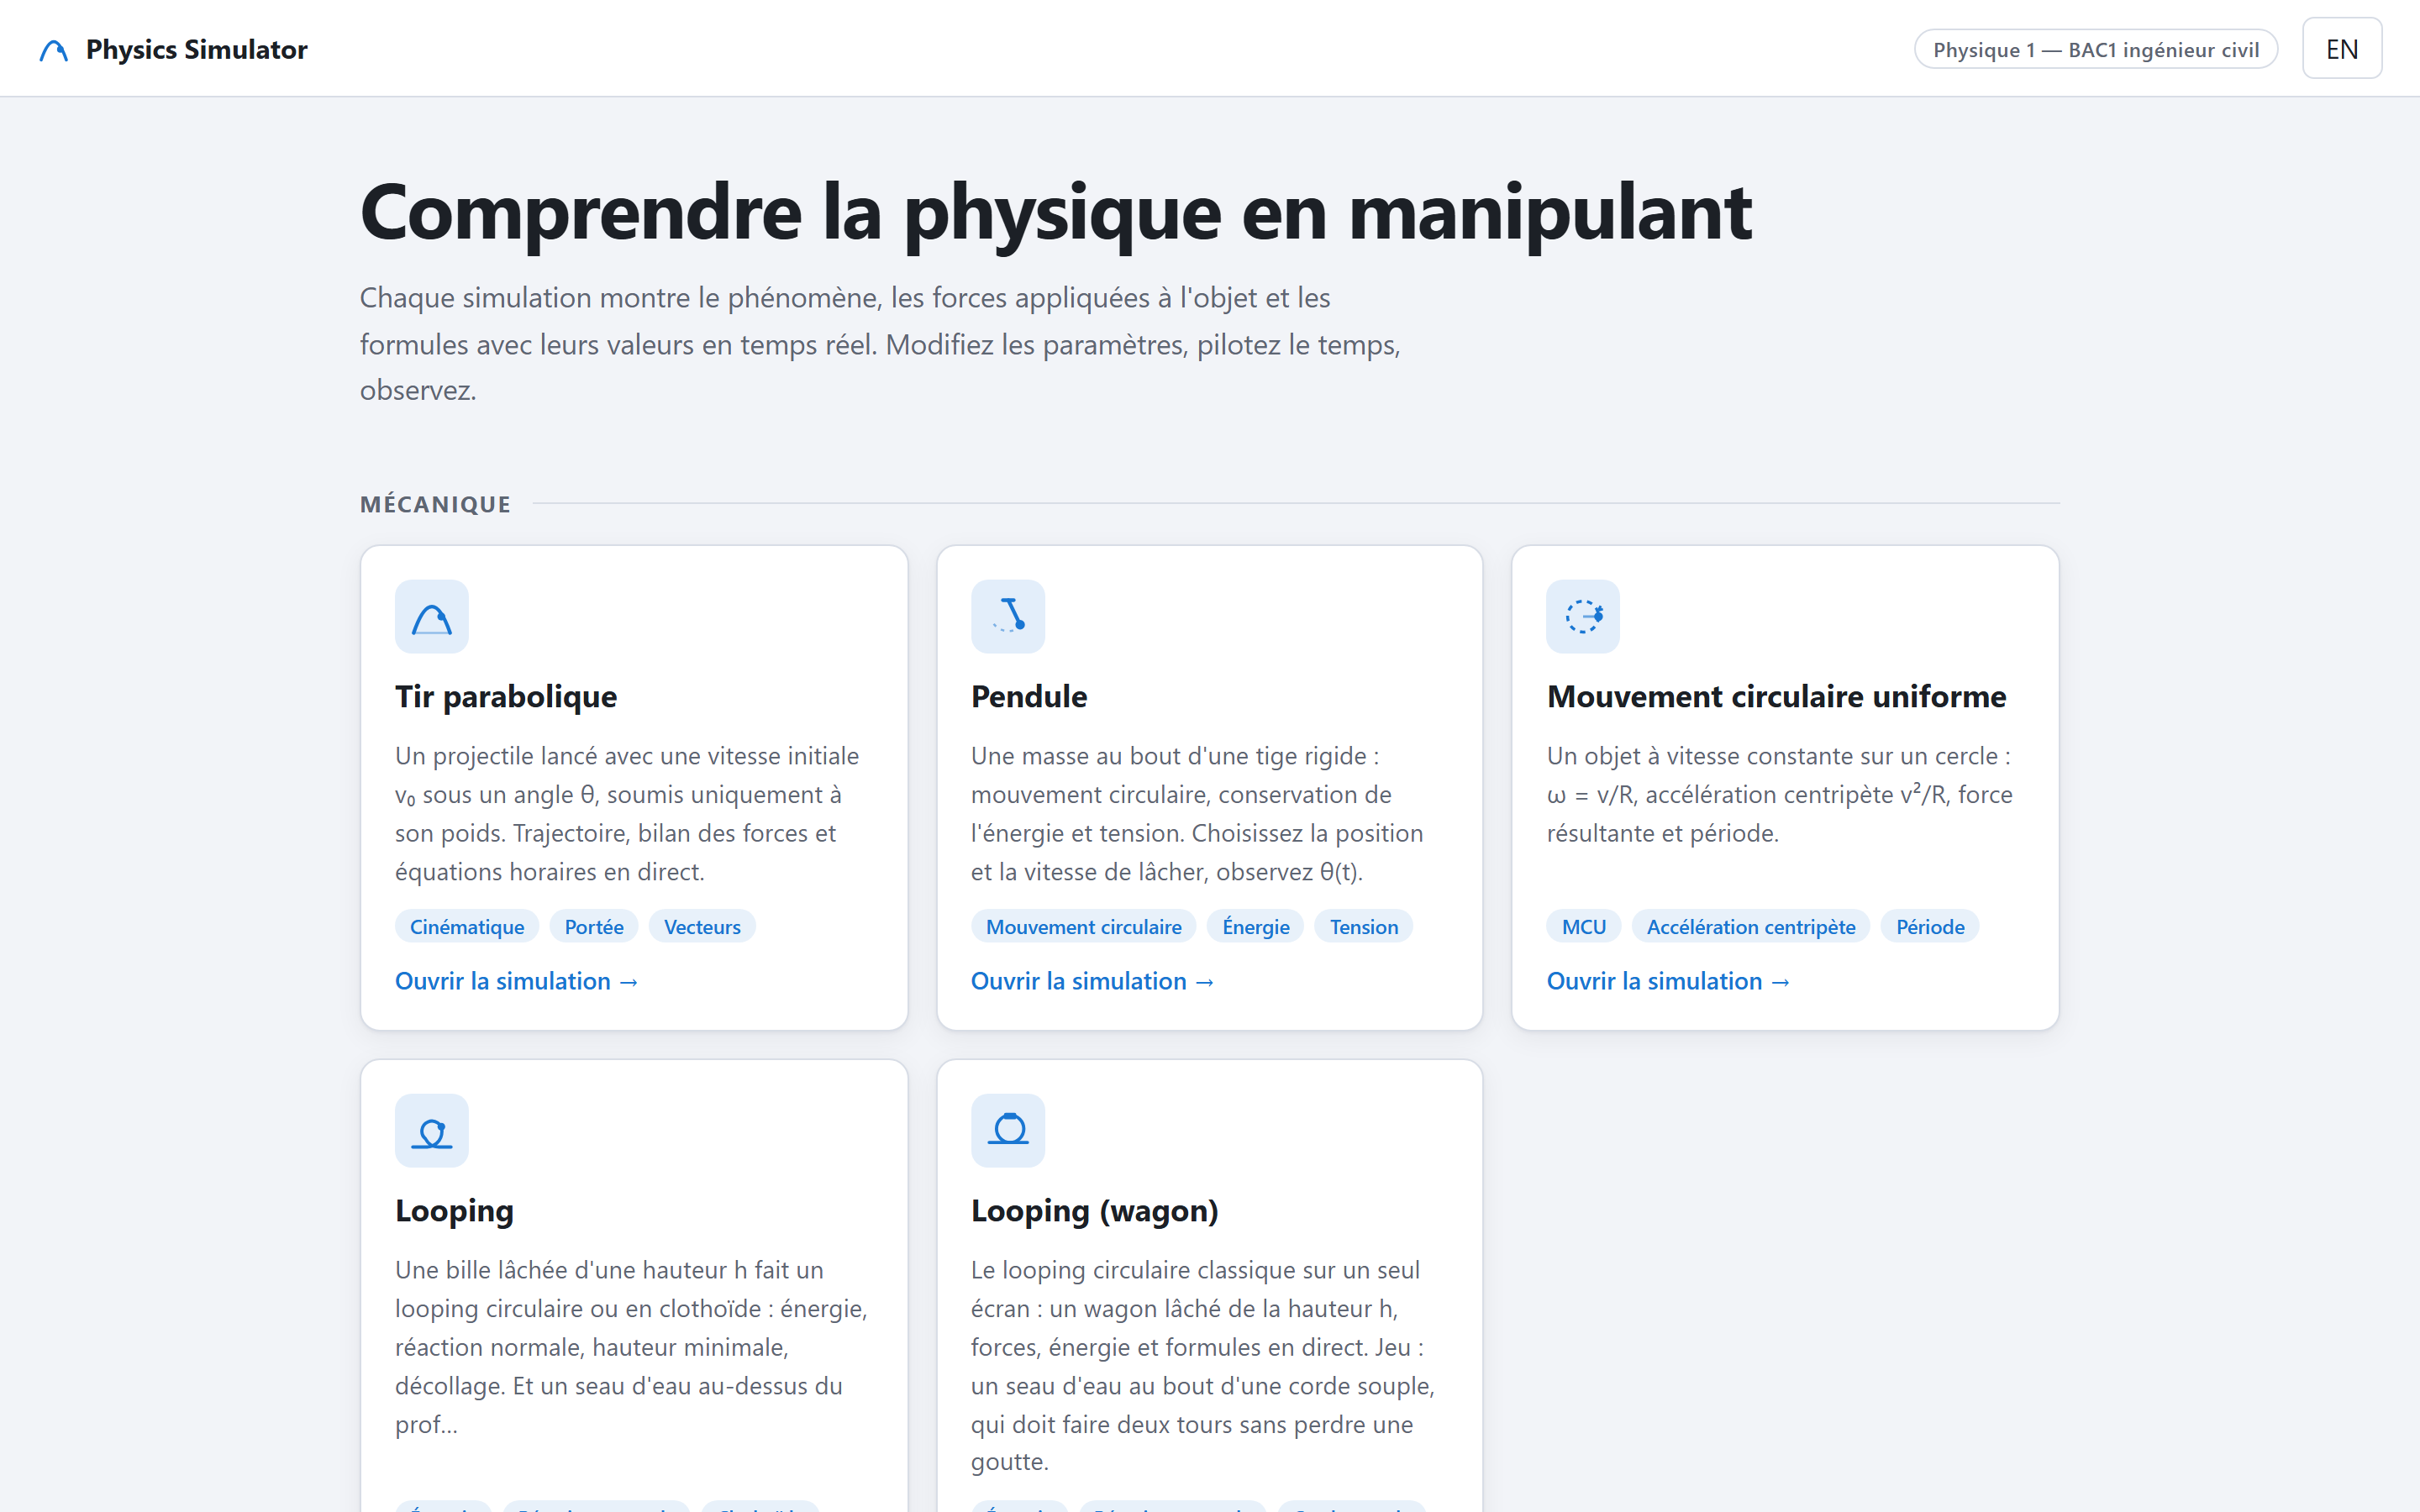
\includegraphics[width=0.85\linewidth]{figures/captures/accueil.png}
  \caption{Page d'accueil du site : un exercice par carte, regroupés par thème.}
  \label{fig:intro-accueil}
\end{figure}

\section{Plan du mémoire}

\begin{arediger}{½ page}
La partie~I fait l'état de l'art (difficultés des étudiants, simulations et
apprentissage, ludification, méthodes numériques, IA pour le développement).
La partie~II décrit la réalisation (cahier des charges et méthodologie,
architecture et exercices, jeu du seau d'eau, validation). La partie~III
présente le protocole, les résultats et leur discussion. Une conclusion
ouvre les perspectives.
\end{arediger}
